 \providecommand{\main}{../../..}
\documentclass[\main/main.tex]{subfiles}
\begin{document}
\section{Teorema Minkowsky-Weyl}

\begin{minipage}{\textwidth}
  \begin{minipage}{.83\textwidth}
    \flushleft
    \begin{theorem}[Minkowsky-Weyl, forma sintetica]
      Ogni punto di un politopo si può ottenere come combinazione convessa dei suoi vertici.
    \end{theorem}
  \end{minipage}\hfill
  \begin{minipage}{0.15\textwidth}\center
    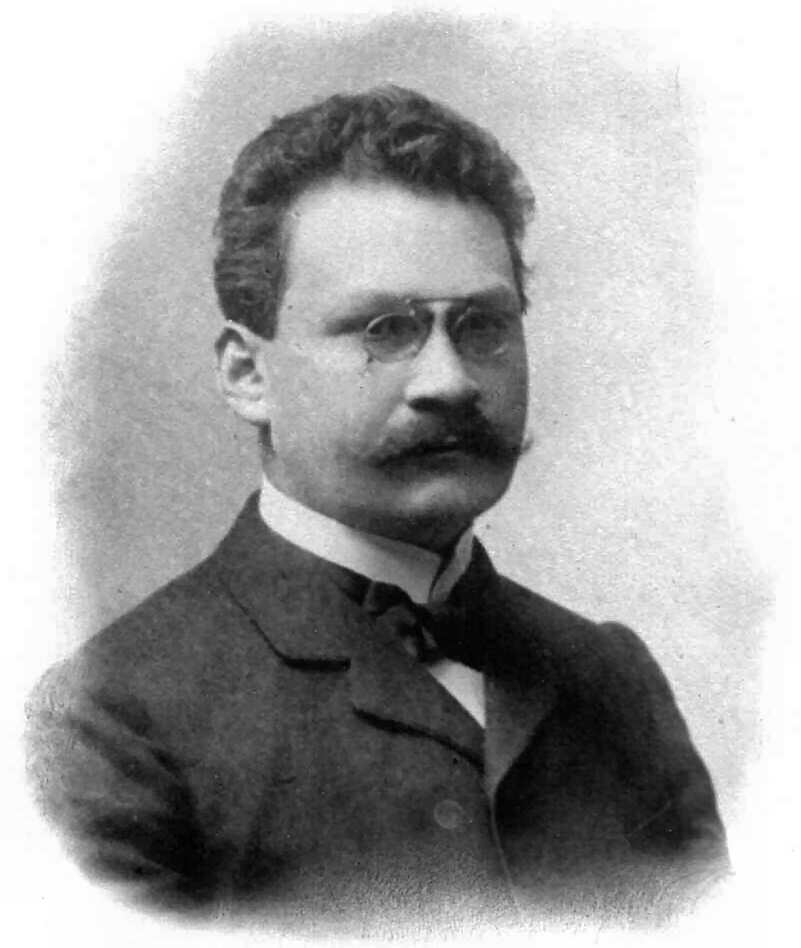
\includegraphics[width=\textwidth]{random/mink}
  \end{minipage}
\end{minipage}

\end{document}